\documentclass[preview]{standalone}

\usepackage{amsmath}
\usepackage{amssymb}
\usepackage{bettelini}
\usepackage{stellar}
\usepackage{definitions}
\usepackage{makecell}
\usepackage{tikz}
\usetikzlibrary{arrows,matrix}

\begin{document}

\id{cyclid-groups}
\genpage

\section{Cyclid groups}

\begin{snippetdefinition}{cyclic-group-definition}{Cyclic Group}
    Let \(G\) be a \group. For any element \(g\) in \(G\),
    the \textit{cyclic group} is the \group generated by \(g\).
\end{snippetdefinition}

\begin{snippetcorollary}{cyclic-is-abelian}{Cyclic groups are abelian}
    Let \(G\) be a \group. If \(G\) is \cyclicgroup[cyclic], then it is \abeliangroup[abelian].
\end{snippetcorollary}

\begin{snippetproof}{cyclic-is-abelian-proof}{cyclic-is-abelian}{Cyclic groups are abelian}
    A generated \subgroup is \abeliangroup[abelian] \ifandonlyif
    the elements of its generator commute. Since the \cyclicgroup
    has only one element, it commutes with itself.
\end{snippetproof}

\begin{snippettheorem}{subgroups-of-cyclic-are-cyclic}{Subgroups of cyclic groups}
    Any \subgroup of a \cyclicgroup is \cyclicgroup[cyclic].
\end{snippettheorem}

\begin{snippetproof}{subgroups-of-cyclic-are-cyclic-proof}{subgroups-of-cyclic-are-cyclic}{Subgroups of cyclic groups}
    Let \((H, \circ) \subgroupleq (G, \circ) = \langle g \rangle\).
    The \subgroup \(H\) is formed by (some) power of \(g\). We consider the following subset:
    \[
        S = \{ n \in \integers \suchthat g^n \in H \}
    \]
    We have that \(0 \in S\) as \(g^0 = 1 \in H\).
    If \(S = \{0\}\), \(H=\{1\}\) and we are done (it is generated by \(1\)).
    If \(S \neq \{0\}\), there are \(n\neq 0 \in S\).
    This means that \(g^n \in H\).
    Since \(g^n \in H\), we also have \(g^{-n} \in H\), meaning \(-n\in S\).
    Since \(n \neq 0\), either \(n\) or \(-n\) is positive.
    This implies that \(S\) contains some positive integers.
    Let \(d\) be the smallest positive integer in \(S\).
    This means that \(g^d \in H\) and if \(0<k<d\), then \(g^k \notin H\).
    We now show that \(g^d\) generates \(H\), meaning that every element of \(H\)
    is a power of \(g^d\). The powers of \(g^d\)
    are of the form \(g^{dn}\) with \(n \in \integers\).
    Let \(g^m \in H\). We want to show that \(m=dn\) for some \(n\).
    We thus divide \(m\) by \(d\). We get
    \begin{align*}
        m &= dq + r \qquad 0\leq r < d \\
        g^m &= g^{dq+r} = {(g^d)}^r \circ g^r
    \end{align*}
    We want to show that \(g^r = 1\). Now, \(g^r = {(g^d)}^{-q} \circ g^m\).
    Both terms are in \(H\), so \(g^r \in H\). By definition of \(d\), \(r=0\)
    since we cannot have \(0 < r < d\) such that \(r\in S\).
    Finally \(g^m = g^{dq}\).
\end{snippetproof}

\begin{snippetproposition}{cyclic-group-powers}{Cyclic groups powers}
    Let \(G\) be a \group. For any element \(g\) in \(G\),
    the \cyclicgroup
    \[
        \langle g \rangle = \{ g^k \suchthat k \in \naturalnumbers \}
    \]
\end{snippetproposition}

\subsection{Period of a cyclic group}

\begin{snippetdefinition}{cyclic-group-period-definition}{Cyclic group period}
    Let \((G, \circ) = \langle g \rangle\) be a \cyclicgroup.
    The \emph{period} of \(g\)
    is the smallest positive integer \(d\) such that \(g^d = 1\)
    and is denoted as \(|g|\).
    We define \(|g| = \infty\) if all the powers of \(g\) are distinct.
\end{snippetdefinition}

\begin{snippettheorem}{cyclic-group-periodic-finite}{Finite cyclic group}
    A \cyclicgroup is \cyclicperiod[periodic] \ifandonlyif it is finite.
    % TODOURGENT or has finite period
    The \cyclicperiod is the order of the \group.
\end{snippettheorem}

\begin{snippetproof}{cyclic-group-periodic-finite-proof}{cyclic-group-periodic-finite}{Finite cyclic group}
    Let \((G, \circ)\) be a \cyclicgroup. We know that
    \[
        (G, \circ) = \{ g^n \suchthat n \in \integers \}
    \]
    Let \(m,n \in\integers\) such that \(m\neq n\).
    In the case where \(g^m \neq g^n\), the \group is infinite.
    If this does not happen, there exist \(m\) and \(n\) such that \(g^m = g^n\).
    Without loss of generality, assume \(n>m\).
    We thus have \(g^{n-m} = g^n \circ g^{-m} = g^m \circ g^{-m} = 1\).
    Thus, there exist \(n-m>0\) such that \(g^{n-m} = 1\). This always happens
    when two different powers give the same element.
    Let \(d\) be the smallest positive integer such that
    \(g^d = 1\).
    We now show that \(g^n = g^k\) \ifandonlyif \(h \equiv k \pmod{d}\).
    We divide \(h-k\) by \(d\), and we get
    \begin{align*}
        h-k = qd + r \qquad 0 \leq r < d
    \end{align*}
    We thus have \(g^h = g^k \circ g^{qd} \circ g^r\).
    Since \(g^qd = 1^q = 1\), \(g^h = g^k \circ g^r\).
    Thus, \(g^h = g^k\) \ifandonlyif \(g^r = 1\),
    which only happens when \(r=0\) by the definition of \(d\),
    meaning \(h\equiv k \pmod{d}\).
    It follows that \(\langle g \rangle\) is finite and it contains
    exactly \(d\) elements.
    We may also note that \(|g| = 1 \iff g=1\).
\end{snippetproof}

\subsection{Subgroups of infinite cyclic groups}

\begin{snippetproposition}{subgroups-of-infinite-cyclic-groups}{Subgroups of infinite cyclic groups}
    The \cyclicgroup[cyclic] \subgroup[subgroups]
    of an infinite \cyclicgroup are infinite, except
    for the trivial case.
\end{snippetproposition}

\begin{snippetproof}{subgroups-of-infinite-cyclic-groups-proof}{subgroups-of-infinite-cyclic-groups}{Subgroups of infinite cyclic groups}
    Let \((G, \circ) = \langle g \rangle\)
    where \(|g| = \infty\).
    We know that the \subgroup[subgroups] are of the form
    \(\langle g^n \rangle\) for \(n\in\integers\).
    We want to study \(|g^n|\).
    We have that \({(g^n)}^k = 1\) \ifandonlyif \(g^nk = 1\),
    which happens \ifandonlyif \(nk=0\).
    if \(n=0\), this happens for every \(k\) (\(\langle g^n \rangle\) is the trivial case).
    If \(n\neq 0\), this happens \ifandonlyif \(k=0\), meaning \(|g^n| = \infty\).
\end{snippetproof}

\begin{snippetproposition}{infinite-cyclic-groups-comparison}{}
    Let \(\langle g \rangle = (G, \circ)\) be a \cyclicgroup where \(|g|=\infty\).
    We have that
    \[\langle g^n \rangle \subgroupleq \langle g^m \rangle \iff m \divides n\]
    and
    \[
        \langle g^n \rangle = \langle g^m \rangle \iff m=n \lor m=-n
    \]
    In particular, \((G, \circ) = \langle g \rangle = \langle g^{-1} \rangle\).
\end{snippetproposition}

\begin{snippetproof}{infinite-cyclic-groups-comparison-proof}{infinite-cyclic-groups-comparison}{}
    We now want to compare \(\langle g^n \rangle\)
    and \(\langle g^m \rangle\). The two are the same if
    if the generator is in both \subgroup[subgroups].
    We have that \(\langle g^n \rangle \subgroupleq \langle g^m \rangle\)
    \ifandonlyif there exist \(h\in\integers\) such that \(g^n = {(g^m)}^h = g^{mh}\).
    Since \(|g| = \infty\), this happens \ifandonlyif \(n=mh\), that is \ifandonlyif
    \(m\divides n\).
\end{snippetproof}

\begin{snippet}{cyclic-subgroups-illustration}
    \begin{center}
        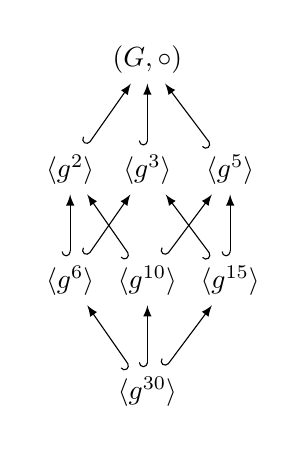
\begin{tikzpicture}[scale=2]
            \matrix [matrix of math nodes, row sep = 0.8cm]
                {
                                      & |(1)| {(G, \circ)}               &  \\
                |(2)| {\langle g^{2}\rangle} & |(3)| {\langle g^{3}\rangle}   & |(5)|  {\langle g^{5}\rangle} \\
                |(6)| {\langle g^{6}\rangle} & |(10)| {\langle g^{10}\rangle} & |(15)| {\langle g^{15}\rangle} \\
                                      & |(30)| {\langle g^{30}\rangle} &  \\
                };
            \draw[right hook-latex] (2)--(1);
            \draw[right hook-latex] (3)--(1);
            \draw[right hook-latex] (5)--(1);

            \draw[right hook-latex] (6)--(2);
            \draw[right hook-latex] (10)--(2);

            \draw[right hook-latex] (6)--(3);
            \draw[right hook-latex] (15)--(3);

            \draw[right hook-latex] (10)--(5);
            \draw[right hook-latex] (15)--(5);

            \draw[right hook-latex] (30)--(6);
            \draw[right hook-latex] (30)--(10);
            \draw[right hook-latex] (30)--(15);

        \end{tikzpicture}
    \end{center}
\end{snippet}

\plain{This diagram is a lattice.}

\end{document}
